\section{Introduction}
\label{sec:intro}
Arc discharges are widely used in welding, cutting and thermal spraying, and in recent years they have found new applications in plasma pyrolysis, advanced material synthesis and metallurgical reduction \cite{boulos2023handbook,aghayee2024plasma,zhang2017synthesis,mohanta2026electrical}. A typical arc discharge consists of a hot quasi-neutral plasma, referred to as the bulk plasma, which is millimeters to centimeters in size and in which convection, thermal conduction, Joule heating and radiation interact under conditions often close to local thermodynamic equilibrium (LTE). Over a region of a millimeter from the electrodes, which is often referred to as the near-electrode or electrode region/layer, the interaction with the electrodes results in a highly non-uniform plasma with strong gradients in the species densities and temperatures. Very close to the electrodes (at sub-micrometer distances), charge separation develops, quasi-neutrality breaks down and strong electric fields arise. 

Because of the high temperatures (\(\sim\)20\,000~K) and  very small length scales compared with macroscopic dimensions, analyzing an arc discharge through experiments is difficult, and therefore there is a strong dependence on computational models. Computational models solve a set of governing equations and boundary conditions to describe a plasma phenomenon. Plasma phenomena are, however, characterized by a wide range of length scales in arc discharges. Resolving these wide range of length scales over the entire discharge is neither computationally practical nor necessary for most applications. For example, Poisson's equation, which governs the charge separation and the electric field near the electrodes, need not be solved in the bulk plasma, where quasi-neutrality holds. Conversely, the electrode regions are thin compared with the flow and geometric scales of the arc, so convection, electrode jets and the electrode geometry can be neglected there. These layers are governed by diffusion, reactions and sheath effects. Arc models therefore typically combine a quasi-neutral model of the bulk plasma with a separate near-electrode model. Several strategies have been adopted for modelling the bulk plasma, and the choice determines what the near-electrode model must describe.

\emph{(i) Local thermodynamic equilibrium.} Measurements of the species temperatures and the electron density indicate that the arc core is generally close to LTE \cite{pokrzywka1996spectroscopic,murphy1992laser,tanaka1999plasma}. In an LTE model, electrons and heavy particles are assumed to have a single temperature \(T\) with Maxwellian velocity distributions and Boltzmann excitation. The plasma state and its properties are determined from the Saha equation and Dalton's law. The governing equations typically consist of mass, momentum and energy conservation together with current continuity \cite{lago2004numerical,freton2000comparison,Hsu1983,korsipati2026fast}. These models are computationally efficient because the species densities and transport properties need not be solved for and follow from the local temperature and pressure. An LTE bulk model, however, requires a near-electrode model that captures the separation of the electron and heavy-particle temperatures, the departure from Saha equilibrium, the breakdown of quasi-neutrality and the formation of the space-charge sheath \cite{Almeida2008,almeida2009investigating,semenov2016numerical}.

\emph{(ii) Two-temperature models.} Two-temperature (2T) models treat electrons and heavy particles as separate Maxwellian populations at temperatures \(T_e\) and \(T_h\), coupled through elastic energy exchange. In two-temperature equilibrium (2T-EQ) models, the composition is, in addition, obtained from a generalized Saha relation for \(T_e\neq T_h\). Hsu and Pfender \cite{HsuPfender1983b} showed that \(T_e\approx T_h\) in the high-density arc core, whereas the temperatures separate significantly in the low-density fringes and near the anode. The generalized Saha closure is not unique, however, and different formulations can predict electron densities that differ by up to an order of magnitude once \(T_e/T_h\) departs from unity \cite{Rat2008}. Freton \textit{et al.} \cite{Freton2012} have further shown that several published formulations distribute the ionization term and the reactive thermal conductivity inconsistently between the electron and heavy-particle energy equations. A 2T bulk model still requires a near-electrode model that captures the ionization layer, or presheath, where Saha equilibrium is violated, as well as the breakdown of quasi-neutrality and the formation of the space-charge sheath \cite{benilov1995model,schmitz2002analysis}.

\emph{(iii) Nonequilibrium models.} Fully nonequilibrium models abandon equilibrium closures such as LTE and Saha equilibrium and let the plasma composition and the electron and heavy-particle temperatures evolve independently. They typically include multicomponent species transport and separate electron and heavy-particle energy equations. Examples are the nonequilibrium arc models of Haidar \cite{haidar1999non}, Gonzalez \textit{et al.} \cite{gonzalez2000decay} and Amakawa \textit{et al.} \cite{amakawa1998anode}. Because they resolve departures from equilibrium directly, these models can describe the transition from the LTE-like bulk plasma to the strongly nonequilibrium electrode region. The space-charge sheath, however, is still treated separately, by a sheath model matched to the quasi-neutral plasma \cite{baeva2016novel}.

A widely used near-electrode modelling approach treats the ionization layer, or presheath, as a collisional region and couples it to a collisionless sheath model \cite{DinulescuPfender1980,hsu1983analysis,schmitz2002analysis,benilov1995model}. This avoids solving the stiff Poisson equation across the sheath. Almeida, Benilov and Naidis \cite{Almeida2008}, however, estimated the number of collisions that an ion undergoes while crossing the cathode space-charge sheath of an atmospheric-pressure argon arc and found it to be of order unity rather than small, so that, strictly speaking, the collisionless-sheath assumption is not justified. A kinetic (particle-in-cell/Monte Carlo collision) study of the near-cathode region by Sun \textit{et al.} \cite{sun2022unified} likewise supports this view. At the anode, however, Semenov \textit{et al.} \cite{semenov2016numerical} showed that the common collisionless sheath model, in which the ion velocity at the sheath edge is set to the Bohm velocity, fails. A physically consistent electrode model for high-pressure arcs should therefore account for collisional ion transport within the sheath.

The alternative is \emph{unified modelling}, in which a single set of governing equations, including Poisson's equation, is solved \rev{from the electrode surface through the sheath to the bulk plasma, with no matching between sub-regions} \cite{Almeida2008,semenov2016numerical,sun2022unified,sitaraman2026elucidating}. Ion collisions in the sheath are then accounted for by construction. Because a unified model captures both thermal and ionization nonequilibrium, it can be matched directly to an LTE model of the bulk plasma. In addition, this approach requires no prior knowledge of the direction of the electric field. Field reversals, and changes in the sign of the potential drop near the anode, have been reported in atmospheric-pressure arcs, depending on factors such as the attachment mode, the current density and electrode ablation \cite{SandersPfender1984,nemchinsky2016anode,heberlein2010anode,baeva2016novel}. When \rev{these equations are} solved self-consistently across the near-electrode region, the potential structure of the sheath and its polarity emerge from the solution instead of being assumed a priori. Unified models are, however, computationally expensive, because the mesh must resolve the very small length scales of the sheath. Consequently, their application to arc discharges has largely been restricted to one-dimensional calculations extending from the electrode into the bulk plasma \cite{Almeida2008,almeida2009investigating,krivtsun2025model,semenov2016numerical}.

In this paper we adopt the decomposition described above, treating the quasi-neutral bulk plasma and the near-electrode region with separate models (figure~\ref{fig:schematic}), and present a transient one-dimensional unified near-electrode model. The near-electrode model is \rev{unified in this sense, with drift-diffusion fluxes for the charged species coupled to Poisson's equation. It} determines the charged-particle distributions, the species fluxes, the sheath voltage drop and the heat flux to the electrode simultaneously. The same system of equations is solved continuously from the quasi-neutral bulk plasma at one end of the domain, through the near-electrode transition region, and into the sheath. In previous one-dimensional unified models \cite{Almeida2008,krivtsun2025model,almeida2009investigating,semenov2016numerical}, the bulk-plasma state was obtained from the asymptotic arc column, assuming a uniform plasma in which Joule heating is balanced by radiative losses, with no radial heat transfer. In the present model, the state of the bulk plasma at the outer boundary is instead supplied from measurements or from an LTE model of the arc, and the radial heat loss of the column is included, which can be important, especially in the near-cathode region, where the temperatures are high \cite{boulos2023handbook,elenbaas1935ahnlichkeitsgesetze}. Gradients of the plasma properties, which drive ambipolar diffusion and heat fluxes, may exist at this boundary. The only requirement is that the plasma there be reasonably close to LTE. In this way, the model can directly receive the plasma state from an LTE model which facilitates the coupling. The near-electrode model and its numerical implementation are described in Section~\ref{sec:model}. The model is validated in Section~\ref{sec:validation} and applied to the near-cathode and near-anode layers of a high-intensity argon arc in Section~\ref{sec:results}.

\begin{figure}[!htbp]
\centering
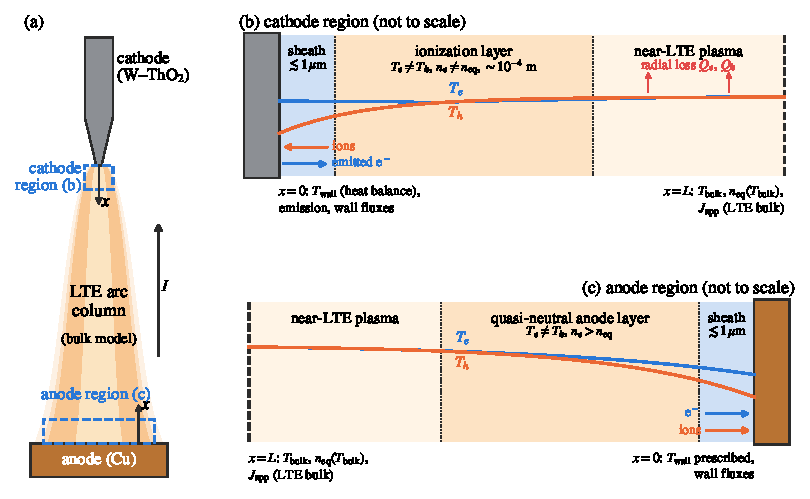
\includegraphics[width=\textwidth]{figures/schematic/arc_schematic.pdf}
\caption{Schematic of the arc discharge and the modeled near-electrode regions.}
\label{fig:schematic}
\end{figure}
